\section{Tasya Wiendhyra / 1164086}
\subsection{Teori}
\subsubsection{Jelaskan kenapa teks harus di lakukan tokenizer. dilengkapi dengan ilustrasi atau gambar}
Untuk memudahkan mesin memahami maksud dari apa yang kita inginkan dalam machine learning, kata pada teks disebut token, dan proses vektorisasi dari bentuk kata ke dalam token tersebut disebut tokenizer dan tokenizer akan merubah sebuah teks menjadi simbol, kata, ataupun biner dan bentuk lainnya kedalam token. Untuk lebih jelasnya perhatikan ilustrasi berikut. Disini saya mempunyai sebuah kalimat yaitu "Nama Saya Tasya Wiendhyra" maka ketika kita lakukan proses tokenizer maka akan berubah menjadi ['Nama', 'Saya', 'Tasya', 'Wiendhyra].

\subsubsection{Jelaskan konsep dasar K Fold Cross Validation pada dataset komentar Youtube pada kode listing \ref{lst:7.0}.dilengkapi dengan ilustrasi atau gambar} 
\begin{lstlisting}[caption=K Fold Cross Validation,label={lst:7.0}]
kfold = StratifiedKFold(n_splits=5)
splits = kfold.split(d, d['CLASS'])
\end{lstlisting}

StartifiedKFold berisikan presentasi sampel untuk setiap kelas. Dimana dalam ilustrasi ini sampel dibagi menjadi 5 dalam setiap class nya. Kemudian sampel tadi akan dimasukan kedalam class dari dataset youtube tadi.

Untuk ilustrasi lebih jelasnya, ada pada gambar berikut :
\begin{figure}[ht]
\centering
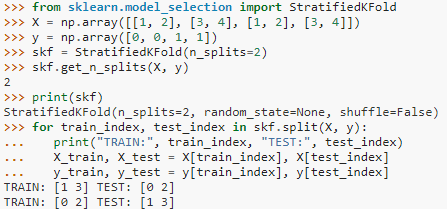
\includegraphics[scale=0.5]{figures/Chapter 7/1164086/Teori/chapter7tasya1.png}
\caption{Ilustrasi KFold Cross Tasya}
\label{Teori}
\end{figure}

\subsubsection{Jelaskan apa maksudnya kode program for train, test in splits.dilengkapi dengan ilustrasi atau gambar.} 
Maksudnya yaitu untuk menguji apakah setiap data pada dataset sudah di split dan tidak terjadi penumpukan. Yang dimana maksudnya di setiap class tidak akan muncul id yang sama. Ilustrasinya misalkan kita memiliki 4 baju dengan model yang berbeda. Kemudian kita bagikan kedua anak, tentunya setiap anak yang menerima baju tidak memiliki baju yang sama modelnya.

\subsubsection{Jelaskan apa maksudnya kode program \emph{train\_content = d['CONTENT'].iloc[train\_idx]} dan \emph{test\_content = d['CONTENT'].iloc[test\_idx]}. dilengkapi dengan ilustrasi atau gambar}

Maksudnya yaitu mengambil data pada kolom atau index CONTENT yang merupakan bagian dari train\_idx dan test\_idx. Ilustrasinya, ketika data telah diubah menjadi train dan test maka kita dapat memilihnya untuk ditampilkan pada kolom yang diinginkan.

\subsubsection{Soal No. 5 Jelaskan apa maksud dari fungsi \emph{tokenizer = Tokenizer(num\_words=2000)} dan \emph{tokenizer.fit\_on\_texts(train\_content)}, dilengkapi dengan ilustrasi atau gambar} 
Dimana variabel tokenizer akan melakukan vektorisasi kata menggunakan fungsi Tokenizer yang dimana jumlah kata yang ingin diubah kedalam bentuk token adalah 2000 kata. Dan untuk \emph{tokenizer.fit\_on\_texts(train\_content)} maksudnya kita akan melakukan fit tokenizer hanya untuk dat trainnya saja tidak dengan data test nya untuk kolom CONTENT. Ilustrasinya, Jadi, jika Anda memberikannya sesuatu seperti, "Kucing itu duduk di atas tikar." Ini akan membuat kamus s.t. word\_index ["the"] = 0; word\_index ["cat"] = 1 itu adalah kata -> kamus indeks sehingga setiap kata mendapat nilai integer yang unik.

\subsubsection{Jelaskan apa maksud dari fungsi \emph{d\_train\_inputs = tokenizer.texts\_to\_matrix(train\_content, mode='tfidf')} dan \emph{d\_test\_inputs = tokenizer.texts\_to\_matrix(test\_content, mode='tfidf')}, dilengkapi dengan ilustrasi kode dan atau gambar} 


Maksudnya yaitu untuk variabel d\_train\_inputs akan melakukan tokenizer dari bentuk teks ke matrix dari data train\_content dengan mode matriksnya yaitu tfidf begitu juga dengan variabel d\_test\_inputs untuk data test. Berikut gambar ilustrasinya
\begin{figure}[ht]
\centering
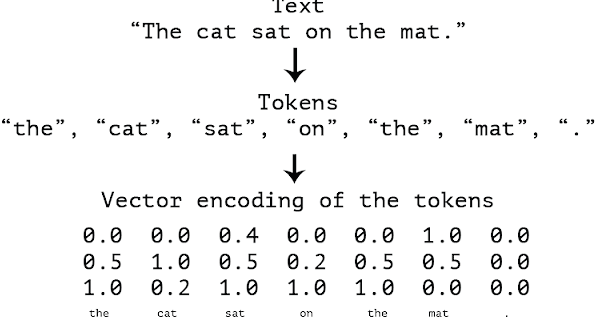
\includegraphics[scale=0.5]{figures/Chapter 7/1164086/Teori/chapter7tasya2.png}
\caption{Ilustrasi Text To Matrix Tasya}
\label{Teori}
\end{figure}

\subsubsection{Jelaskan apa maksud dari fungsi \emph{d\_train\_inputs = d\_train\_inputs/np.amax(np.absolute(d\_train\_inputs))} dan \emph{d\_test\_inputs = d\_test\_inputs/np.amax(np.absolute(d\_test\_inputs))}, dilengkapi dengan ilustrasi atau gambar}

Fungsi tersebut akan membagi matrix tfidf tadi dengan amax yaitu mengembalikan maksimum array atau maksimum sepanjang sumbu. Yang hasilnya akan dimasukan kedalam variabel d\_train\_inputs untuk data train dan d\_test\_inputs untuk data test dengan nominal absolut atau tanpa ada bilangan negatif dan koma.
\begin{figure}[ht]
\centering
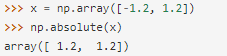
\includegraphics[scale=0.5]{figures/Chapter 7/1164086/Teori/chapter7tasya4.png}
\caption{Ilustrasi np Absolute Tasya}
\label{Teori}
\end{figure}

\subsubsection{Jelaskan apa maksud fungsi dari \emph{d\_train\_outputs = np\_utils.to\_categorical(d['CLASS'].iloc[train\_idx])} dan \emph{d\_test\_outputs = np\_utils.to\_categorical(d['CLASS'].iloc[test\_idx])} dalam kode program, dilengkapi dengan ilustrasi atau gambar}

Dalam variabel d\_train\_output dan d\_test\_outputs akan dilakukan one hot encoding, dimana np\_utilsakan mengubah vektor dengan bentuk integer ke matriks kelas biner untuk kolom CLASS dimana nantinya hanya akan ada dua pilihan yaitu 1 atau 0. 1 untuk spam 0 untuk non spam atau sebaliknya. Berikut gambar ilustrasinya :\\
\begin{figure}[ht]
\centering
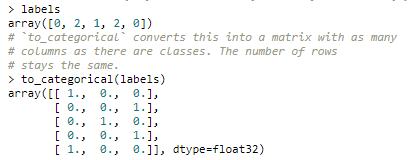
\includegraphics[scale=0.5]{figures/Chapter 7/1164086/Teori/chapter7tasya5.png}
\caption{Ilustrasi One Hot Encoding Tasya}
\label{Teori}
\end{figure}

\subsubsection{Jelaskan apa maksud dari fungsi di listing \ref{lst:7.1}. Gambarkan ilustrasi Neural Network nya dari model kode tersebut.}
\begin{lstlisting}[caption=Membuat model Neural Network,label={lst:7.1}]
       model = Sequential()
       model.add(Dense(512, input_shape=(2000,)))
       model.add(Activation('relu'))
       model.add(Dropout(0.5))
       model.add(Dense(2))
       model.add(Activation('softmax'))
\end{lstlisting}
Penjelasannya sebagai berikut :\\
\begin{itemize}
\item Melakukan pemodelan Sequential
\item Layer pertama dense dari 512 neuron untuk inputan dengan inputan tadi yang sudah dijadikan matriks sebanyak 2000
\item Activationnya menggunakan fungsi relu yaitu jika ada inputan dengan nilai maksimum maka inputan itu yang akan terpilih.
\item Dropout ini untuk melakukan pembobotan, dimana pembobotan hanya dilakukan 50\% saja agar tidak terjadi penumpukan data dari dense inputan tadi
\item Dense 2 mengkategorikan 2 neuron untuk output nya yaitu 1 dan 0.
\item Untuk dense diatas aktivasinya menggunakan fungsi Softmax.
\end{itemize}

Ilustrasinya seperti berikut :\\
\begin{figure}[ht]
\centering
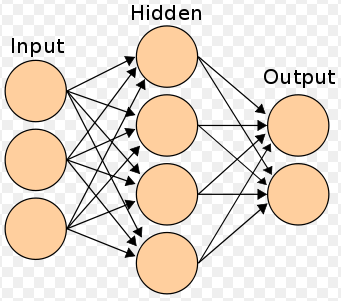
\includegraphics[scale=0.5]{figures/Chapter 7/1164086/Teori/chapter7tasya6.png}
\caption{Ilustrasi Neural Network Pemodelan Tasya}
\label{Teori}
\end{figure}

\subsubsection{Jelaskan apa maksud dari fungsi di listing \ref{lst:7.2} dengan parameter tersebut}
\begin{lstlisting}[caption=Compile model,label={lst:7.2}]
	model.compile(loss='categorical_crossentropy', optimizer='adamax',
	                  metrics=['accuracy'])
\end{lstlisting}
Melakukan peng compile-an dari model Sequential tadi dengan Loss yandengang merupakan fungsi optimisasi skor  menggunakan categorical\_crossentropy , dan menggunakan algoritma adam sebagai optimizer. Adam yaitu algoritma pengoptimalan yang dapat digunakan sebagai ganti dari prosedur penurunan gradien stokastik klasik untuk memperbarui bobot jaringan yang berulang berdasarkan data training.Dengan metrik yaitu fungsi yang digunakan untuk menilai kinerja mode Anda disini menggunakan fungsi accuracy.

\subsubsection{Jelaskan apa itu Deep Learning}
Deep Learning  adalah subbidang machine learning yang berkaitan dengan algoritma yang terinspirasi oleh struktur dan fungsi otak yang disebut jaringan saraf tiruan atau Artificial Neural Networks. Jaringan saraf tiruan, algoritma yang terinspirasi oleh otak manusia, belajar dari sejumlah besar data. Demikian pula dengan bagaimana kita belajar dari pengalaman, algoritma pembelajaran yang mendalam akan melakukan tugas berulang kali, setiap kali sedikit mengubahnya untuk meningkatkan hasilnya.

\subsubsection{Jelaskan apa itu Deep Neural Network, dan apa bedanya dengan Deep Learning}
Deep Neural Network adalah jaringan syaraf tiruan (JST) dengan beberapa lapisan antara lapisan input dan output. DNN menemukan manipulasi matematis yang benar untuk mengubah input menjadi output, apakah itu hubungan linear atau hubungan non-linear. Merupakan jaringan syaraf dengan tingkat kompleksitas tertentu, jaringan syaraf dengan lebih dari dua lapisan. Deep Neural Network menggunakan pemodelan matematika yang canggih untuk memproses data dengan cara yang kompleks.

DNN hanya terdiri dari dua laipsan yaitu input dan output, sedangkan dalam Deep learning kita dapat mendefiniskan layer sebanyak yang kita inginkan atau butuhkan.

\subsubsection{Jelaskan dengan ilustrasi gambar buatan sendiri(langkah per langkah) bagaimana perhitungan algoritma konvolusi dengan ukuran stride (NPM mod3+1) x (NPM mod3+1) yang terdapat max pooling}
Stridenya 3
\begin{itemize}
\item terdapat data seperti berikut 
\begin{figure}[ht]
\centering
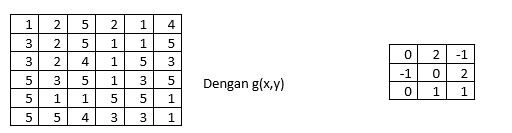
\includegraphics[scale=0.5]{figures/Chapter 7/1164086/Teori/chapter7tasya7.png}
\caption{Algoritma Konvulusi Tasya}
\label{Teori}
\end{figure}
\item Kemudian hitung konvolusi untuk setiap matriksnya seperti berikut :
\begin{itemize}
\item pertama
\begin{figure}[ht]
\centering
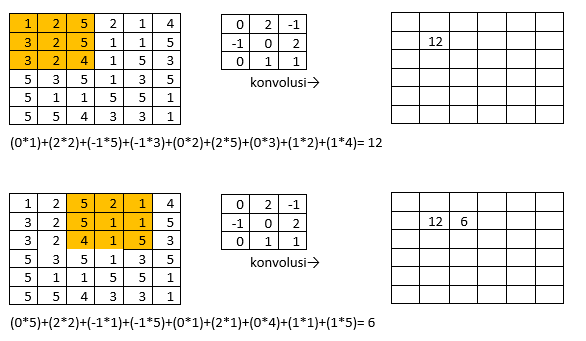
\includegraphics[scale=0.5]{figures/Chapter 7/1164086/Teori/chapter7tasya8.png}
\caption{Algoritma Konvulusi Tasya}
\label{Teori}
\end{figure}
\item Kedua
\begin{figure}[ht]
\centering
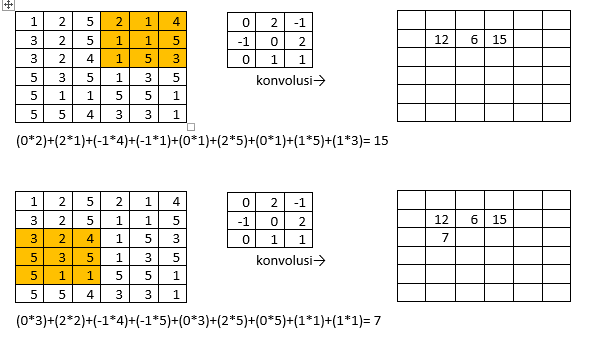
\includegraphics[scale=0.5]{figures/Chapter 7/1164086/Teori/chapter7tasya9.png}
\caption{Algoritma Konvulusi Tasya}
\label{Teori}
\end{figure}
\item Ketiga
\begin{figure}[ht]
\centering
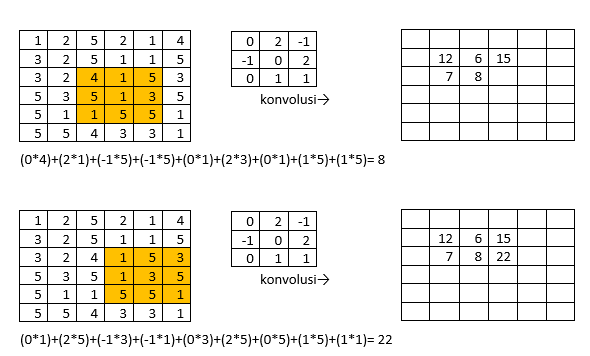
\includegraphics[scale=0.5]{figures/Chapter 7/1164086/Teori/chapter7tasya10.png}
\caption{Algoritma Konvulusi Tasya}
\label{Teori}
\end{figure}
\item Keempat
\begin{figure}[ht]
\centering
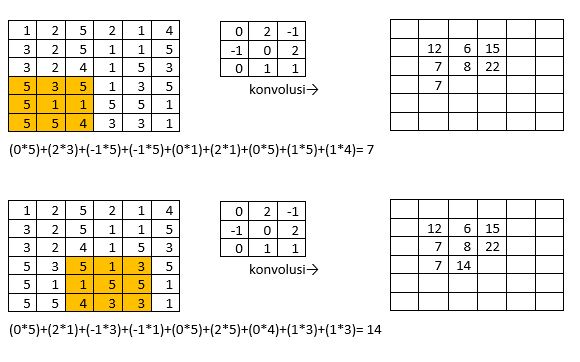
\includegraphics[scale=0.5]{figures/Chapter 7/1164086/Teori/chapter7tasya11.png}
\caption{Algoritma Konvulusi Tasya}
\label{Teori}
\end{figure}
\item Kelima
\begin{figure}[ht]
\centering
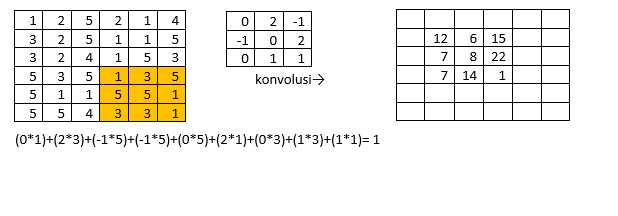
\includegraphics[scale=0.5]{figures/Chapter 7/1164086/Teori/chapter7tasya12.png}
\caption{Algoritma Konvulusi Tasya}
\label{Teori}
\end{figure}
\end{itemize}
\item Didapatkan hasil akhir nilai konvolusi dan juga max poolingnya seperti berikut
\begin{figure}[ht]
\centering
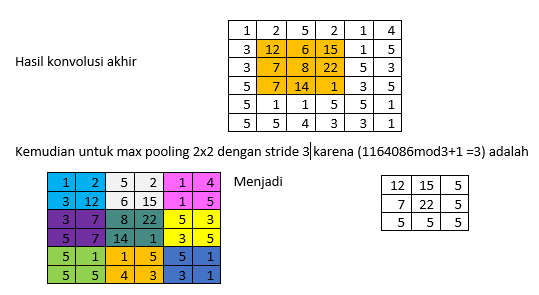
\includegraphics[scale=0.5]{figures/Chapter 7/1164086/Teori/chapter7tasya13.png}
\caption{Algoritma Konvulusi Tasya}
\label{Teori}
\end{figure}
\end{itemize}


\subsection{Praktek}
\subsubsection{No.1 Kode Program Blok \# In 1}
\lstinputlisting[firstline=8, lastline=20]{src/Chapter7/1164086/in1.py}
Keterangannya sebagai berikut :\\
\begin{itemize}
\item Pertama kita akan mengimpor librari csv
\item Dimana dari librai PIL atau Pillow atau Python Imaging Library akan diimpor modul Image yang di inisiasikan sebagain pil\_image. Modul Image menyediakan kelas dengan nama yang sama yang digunakan untuk mewakili gambar PIL. Modul ini juga menyediakan sejumlah fungsi pabrik, termasuk fungsi untuk memuat image dari file, dan untuk membuat image baru.
\item mengimpor librari image dari keras .Yang menghasilkan kumpulan data gambar tensor dengan augmentasi data waktu nyata. Data akan diulang (dalam batch). 
\item Berikut Hasilnya :\\
\begin{figure}[ht]
\centering
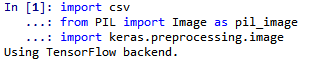
\includegraphics[scale=0.5]{figures/Chapter 7/1164086/Praktek/chapter7tasya14.png}
\caption{Kode Program Blok In 1 Tasya}
\label{Praktek}
\end{figure}
\end{itemize}

\subsubsection{No.2 Kode Program Blok \# In 2}
\lstinputlisting[firstline=8, lastline=20]{src/Chapter7/1164086/in2.py}
Keterangannya sebagai berikut :\\
\begin{itemize}
\item variabel imgs berisikan array kosong
\item Variabel classes berisikan array kosong
\item Membuka file csv dari Folder HSYv2 dengan nama file hasy-data-labels.csv sebagai csvfile
\item Variabel csvreader akan menggunakan fungsi reader pada library csv untuk membaca file csv tadi yang disimpan di csvfile.
\item Dimana variabel i dimuali dari nol.
\item Untuk setiap baris pada  csvreader
\item Jika i lebih besar dari 0
\item Jadi itu akan mengambil contoh Gambar PIL dan mengubahnya menjadi array numpy dengan mengambil data dari HSYv2 dan dimulai dari baris ke nol.
\item Hasil dari variabel img akan dibagi dengan 255.0
\item .append akan membuat list array baru untuk baris 0 baris 2 pada img.
\item Menyimpan setiap class nya  pada baris 2
\item Penambahan i sebanyak 1. 
\item Hasilnya seperti berikut :\\
\begin{figure}[ht]
\centering
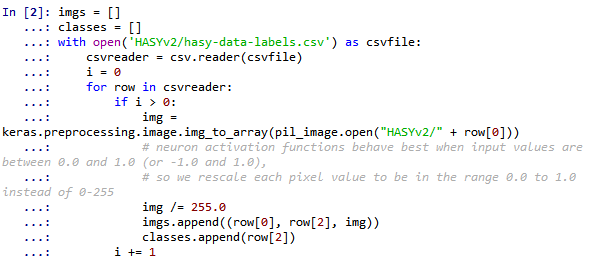
\includegraphics[scale=0.5]{figures/Chapter 7/1164086/Praktek/chapter7tasya15.png}
\caption{Kode Program Blok In 2 Tasya}
\label{Praktek}
\end{figure}
\end{itemize}

\subsubsection{No.3 Kode Program Blok \# In 3}
\lstinputlisting[firstline=8, lastline=20]{src/Chapter7/1164086/in3.py}
Keterangannya sebagai berikut :\\
\begin{itemize}
\item Impor librari Random dari Python
\item Melakukan pengacakan untuk imgs dengan Metode Shuffle  untuk mengocok urutan di tempat. yaitu, mengubah posisi item dalam daftar.
\item Membagi data dari imgs dengan cara mengalikan 80\% dengan jumlah data dari imgs.
\item Untuk data train mengambil hasil dari perhitungan sebelumnya.
\item Untuk data test mengambil sisa dari jumlah yang telah dijadikan data train
\item Hasilnya seperti berikut :
\begin{figure}[ht]
\centering
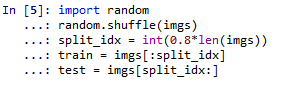
\includegraphics[scale=0.5]{figures/Chapter 7/1164086/Praktek/chapter7tasya16.png}
\caption{Kode Program Blok In 3 Tasya}
\label{Praktek}
\end{figure}
\end{itemize}

\subsubsection{No.4 Kode Program Blok \# In 4}
\lstinputlisting[firstline=8, lastline=20]{src/Chapter7/1164086/in4.py}
Keterangannya sebagai berikut :\\
\begin{itemize}
\item Impor librari Numpy yang di inisiasikan sebagai np
\item Variabel train\_input mengubah input menjadi sebuah array yang diambil dari baris 2, data train.
\item Variabel test\_input mengubah input menjadi sebuah array yang diambil dari baris 2, data test.
\item Variabel train\_output mengubah input menjadi sebuah array yang diambil dari baris 1, data train.
\item Variabel train\_output mengubah input menjadi sebuah array yang diambil dari baris 1, data test.
\item Hasilnya seperti berikut 
\begin{figure}[ht]
\centering
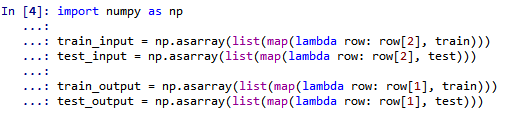
\includegraphics[scale=0.5]{figures/Chapter 7/1164086/Praktek/chapter7tasya17.png}
\caption{Kode Program Blok In 4 Tasya}
\label{Praktek}
\end{figure}
\end{itemize}

\subsubsection{No.5 Kode Program Blok \# In 5}
\lstinputlisting[firstline=8, lastline=20]{src/Chapter7/1164086/in5.py}
Keterangannya sebagai berikut :\\
\begin{itemize}
\item Impor Fungsi LabelEncoder
\item Impor Fungsi OneHotEncoder
\item Berikut hasilnya :\\
\begin{figure}[ht]
\centering
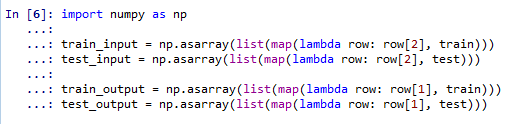
\includegraphics[scale=0.5]{figures/Chapter 7/1164086/Praktek/chapter7tasya18.png}
\caption{Kode Program Blok In 5 Tasya}
\label{Praktek}
\end{figure}
\end{itemize}

\subsubsection{No.6 Kode Program Blok \# In 6}
\lstinputlisting[firstline=8, lastline=20]{src/Chapter7/1164086/in6.py}
Keterangannya sebagai berikut :\\
\begin{itemize}
\item Variabel label\_encoder akan memanggil fungsi LabelEncoder tadi.
\item variabel integer\_encoded akan menggunakan labelencoder untuk melakukan fit pada classes agar berubah datanya menjadi integer.
\item Berikut hasilnya :
\begin{figure}[ht]
\centering
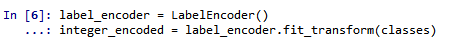
\includegraphics[scale=0.5]{figures/Chapter 7/1164086/Praktek/chapter7tasya19.png}
\caption{Kode Program Blok In 6 Tasya}
\label{Praktek}
\end{figure}
\end{itemize}

\subsubsection{No.7 Kode Program Blok \# In 7}
\lstinputlisting[firstline=8, lastline=20]{src/Chapter7/1164086/in7.py}
Keterangannya sebagai berikut :\\
\begin{itemize}
\item Variabel onehot\_encoder akan memanggil fungsi OneHotEncoder dimana tidak berisikan matriks sparse.
\item Pada variabel integer\_encoded akan diubah bentuknya dimana setiap nilai integer akan direpresentasikan sebagai vektor binari dengan nilai 0 kecuali index dari integer tersebut ditandai dengan 1.
\item Melakukan fit untuk one hot encoder kedalam integer\_encoder.
\item Berikut hasilnya :\\
\begin{figure}[ht]
\centering
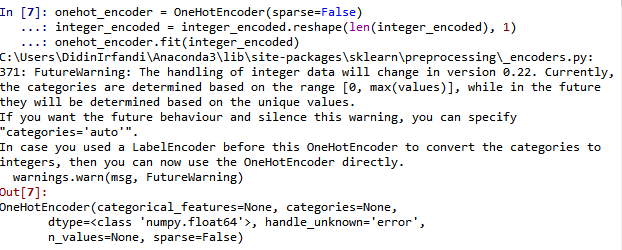
\includegraphics[scale=0.5]{figures/Chapter 7/1164086/Praktek/chapter7tasya20.png}
\caption{Kode Program Blok In 7 Tasya}
\label{Praktek}
\end{figure}
\end{itemize}


\subsection{Penanganan Error}
